\section{Further readings of the sine squared lemma}\label{ch:sin2more}
\label{sec:sin2more}


This section follows the sine squared lemma \eqref{eq:sin2} of Section~\ref{ch:clock} in two directions.

\subsection{The prime side near the critical line}\label{sec:ch10:selberg}

For $\alpha>1$ the integrated lemma is the argument of $\zeta$. In the chart $\theta=\sqrt z$ a unit of $xL(dx)$ at $x$ contributes $\pi^{-1}(1-\cos\theta x)$ to the density, and $\pi^{-1}\int_0^\Theta(1-\cos\theta x)\,d\theta=\pi^{-1}(\Theta-\sin(\Theta x)/x)$, so the prime atoms $\Lambda(n)n^{-\alpha}$ at $x=\log n$ return a term linear in $\Theta$ plus $\pi^{-1}$ times
\[
-\sum_{n\ge2}\frac{\Lambda(n)}{n^\alpha}\frac{\sin(\Theta\log n)}{\log n}=\arg\zeta(\alpha+i\Theta),
\]
on the branch with $\arg\zeta(\alpha)=0$, since $\log\zeta(s)=\sum_n\Lambda(n)n^{-s}/\log n$ for $\re s>1$. Divided by $\pi$, this is $S_{\alpha-1/2}(\Theta)$ in the notation of Section~\ref{sec:ch9:mass}. The series converges absolutely for $\alpha>1$ and diverges for $\alpha<1$, so the function $S$ of Turing's method (Section~\ref{sec:ch5:turing}), at $\alpha=\tfrac12$, is reached only through a smoothing.

Selberg \cite{Selberg46} truncates the Dirichlet series of $\zeta'/\zeta$ smoothly and accounts for the truncation exactly by a sum over the zeros \cite[Section 14.20]{Titchmarsh}. With $\Lambda_x(n)=\Lambda(n)$ for $n\le x$ and $\Lambda_x(n)=\Lambda(n)\log(x^2/n)/\log x$ for $x<n\le x^2$, and for $x>1$ and $s$ different from $1$, from every zero $\rho$ and from every $-2q$,
\begin{equation}\label{eq:ch10:selberg}
\begin{split}
\frac{\zeta'}{\zeta}(s)={}&-\sum_{n\le x^2}\frac{\Lambda_x(n)}{n^s}+\frac{x^{2(1-s)}-x^{1-s}}{(1-s)^2\log x}\\
&+\frac1{\log x}\sum_{q\ge1}\frac{x^{-2q-s}-x^{-2(2q+s)}}{(2q+s)^2}+\frac1{\log x}\sum_\rho\frac{x^{\rho-s}-x^{2(\rho-s)}}{(s-\rho)^2}.
\end{split}
\end{equation}
At $s=\alpha+i\theta$ with $\alpha=\tfrac12+\varepsilon$, a zero $\rho=\beta+i\gamma$ with $\beta<\alpha$ contributes to the last sum a term of modulus about $x^{\beta-\alpha}/(|s-\rho|^2\log x)$. For a line zero at its own ordinate the term is $(x^{-\varepsilon}-x^{-2\varepsilon})/(\varepsilon^2\log x)$, a fraction $x^{-\varepsilon}(1-x^{-\varepsilon})/(\varepsilon\log x)$ of the contribution $1/\varepsilon$ of that zero to $v_\alpha$; we call this the single zero law. The same computation bounds the whole sum. If no zero has real part greater than $\tfrac12$, then $|x^{\rho-s}|=x^{-\varepsilon}$ and $|x^{2(\rho-s)}|=x^{-2\varepsilon}$ for every zero, and every zero contributes $\re(1/(s-\rho))=\varepsilon/|s-\rho|^2$ to $v_\alpha(\theta)$, so that $\sum_\rho|s-\rho|^{-2}=v_\alpha(\theta)/\varepsilon$ by Proposition~\ref{prop:struct}. Hence the bracket $v_\alpha$ computed from Selberg's smoothed prime sum has error at most
\[
\frac{x^{-\varepsilon}+x^{-2\varepsilon}}{\varepsilon\log x}\,v_\alpha(\theta),
\]
which is of order $x^{-\varepsilon}/(\varepsilon^2\log x)$ at a peak, where $v_\alpha$ is about $1/\varepsilon$, and $k$ correct digits at an ordinate need $x^\varepsilon\,\varepsilon\log x\approx10^k$, that is
\[
x\approx10^{k/\varepsilon}
\]
to leading order, with primes up to $x^2$. A zero with $\tfrac12<\beta<\alpha$ gives a term that decays like $x^{\beta-\alpha}$, more slowly than $x^{-\varepsilon}$, and one with $\beta>\alpha$ a term that grows like $x^{2(\beta-\alpha)}$, since then $x^{2(\rho-s)}$ dominates. With $B=\sup_\rho\re\rho$ the error is $O(x^{B-\alpha}/\log x)$ when $B<\alpha$, and when $B>\alpha$ it reaches $x^{2(B-\alpha)+o(1)}$ along a sequence of cutoffs, so that the prime side diverges as $x\to\infty$ if a zero lies to the right of the line $\re s=\alpha$. Selberg's abscissa $\sigma_{x,t}=\tfrac12+2\max(\beta-\tfrac12,2/\log x)$, the maximum over the zeros near height $t$, takes this into account; when none of these zeros lies to the right of $\tfrac12+2/\log x$ it equals $\tfrac12+4/\log x$, where $x^{-\varepsilon}=e^{-4}$ \cite{Selberg46}. Section~\ref{ch:basepoint} meets the same dichotomy without smoothing.

The terms of the zeros to the right of the line $\re s=\alpha$ cannot cancel one another. Suppose that $B>\alpha$, write $E_x(s)$ for the last term of \eqref{eq:ch10:selberg}, the sum over the zeros divided by $\log x$, and put $y=\log x$, $\lambda_\rho=\rho-s$ and $R(y)=y\re E_{e^y}(s)$. Bounding each term by its modulus gives $|R(y)|\le\sum_\rho|s-\rho|^{-2}\big(e^{(B-\alpha)y}+e^{2(B-\alpha)y}\big)$, so for $\re w>2(B-\alpha)$ the Laplace transform $\int_0^\infty e^{-wy}R(y)\,dy$ may be taken term by term, and it is
\[
\frac12\sum_\rho\Big[\frac1{\lambda_\rho^2}\Big(\frac1{w-\lambda_\rho}-\frac1{w-2\lambda_\rho}\Big)+\frac1{\bar\lambda_\rho^2}\Big(\frac1{w-\bar\lambda_\rho}-\frac1{w-2\bar\lambda_\rho}\Big)\Big].
\]
The series converges locally uniformly away from its poles, since $\sum_\rho|\lambda_\rho|^{-2}<\infty$ and $|\lambda_\rho|\to\infty$, and so defines a meromorphic function in the whole plane. A zero $\rho_0$ with $\re\rho_0>(B+\alpha)/2$ gives a pole at $2\lambda_{\rho_0}$, to the right of every pole $\lambda_\rho$ and $\bar\lambda_\rho$; each fraction with a pole there contributes $-\frac12\lambda_{\rho_0}^{-2}$ to the residue, which is therefore not zero. If $R(y)=O(e^{\eta y})$, the Laplace integral converges on $\re w>\eta$ and continues the series holomorphically there, so $\eta\ge2(\re\rho_0-\alpha)$. Letting $\re\rho_0$ tend to $B$, and using the bound on $|R|$, gives $\limsup_{x\to\infty}\log|\re E_x(s)|/\log x=2(B-\alpha)$.

The cutoff interpolates between the zeros and the primes. For $x<\sqrt2$ the prime sum is empty, and as $x\downarrow1$ each remaining term tends to its partial fraction, $1/(1-s)$, $1/(s+2q)$ or $1/(s-\rho)$. The limits cannot be taken inside the sums separately: the sum over $q$ grows like $\frac12\log(1/\log x)$ and the real part of the sum over the zeros falls like $-\frac12\log(1/\log x)$, and only their total, $\zeta'/\zeta(s)-(x^{2(1-s)}-x^{1-s})/((1-s)^2\log x)$, has a limit, $\zeta'/\zeta(s)+1/(s-1)$. Adding the logarithmic derivative of $s\pi^{-s/2}\Gamma(s/2)$ turns this limit into $\xi'/\xi(s)$, whose real part divided by $\pi$ is the density $\rho_\varepsilon(\theta)$, the sum of the kernels of Proposition~\ref{prop:struct}.

Figure~\ref{fig:selberg} tests the formula at $\varepsilon=0.25$, that is $\alpha=\tfrac34$, on $501$ points of $10\le\theta\le60$, against the P\'olya values of $v_{3/4}$. With the primes alone the maximal relative error is $66\%$, $20\%$ and $7\%$ for $x=30$, $300$ and $3000$, attained where $v_{3/4}$ is small, and the maximal absolute errors $1.14$, $0.53$ and $0.23$, attained at peaks over zeros, follow the single zero law, which predicts $1.15$, $0.51$ and $0.23$; the relative errors stay below the bound $(x^{-\varepsilon}+x^{-2\varepsilon})/(\varepsilon\log x)$, which is $0.72$, $0.21$ and $0.077$. Both errors decrease faster than $x^{-\varepsilon}$. Adding the sum over the first $1700$ zeros reduces the error below $1.6\times10^{-7}$, the residual being the zeros above height $2197$. At $\varepsilon=0.005$ ten digits would need $x\approx10^{2000}$, about $e^{4600}$, to leading order (about $e^{4000}$ by the single zero law), while the cost of one P\'olya evaluation does not depend on $\varepsilon$ (Section~\ref{sec:ch6:split}). So the sine squared lemma identifies the Thorin density, but near the line the primes compute it only at a cost exponential in $1/\varepsilon$.

\begin{figure}[htbp]
\centering
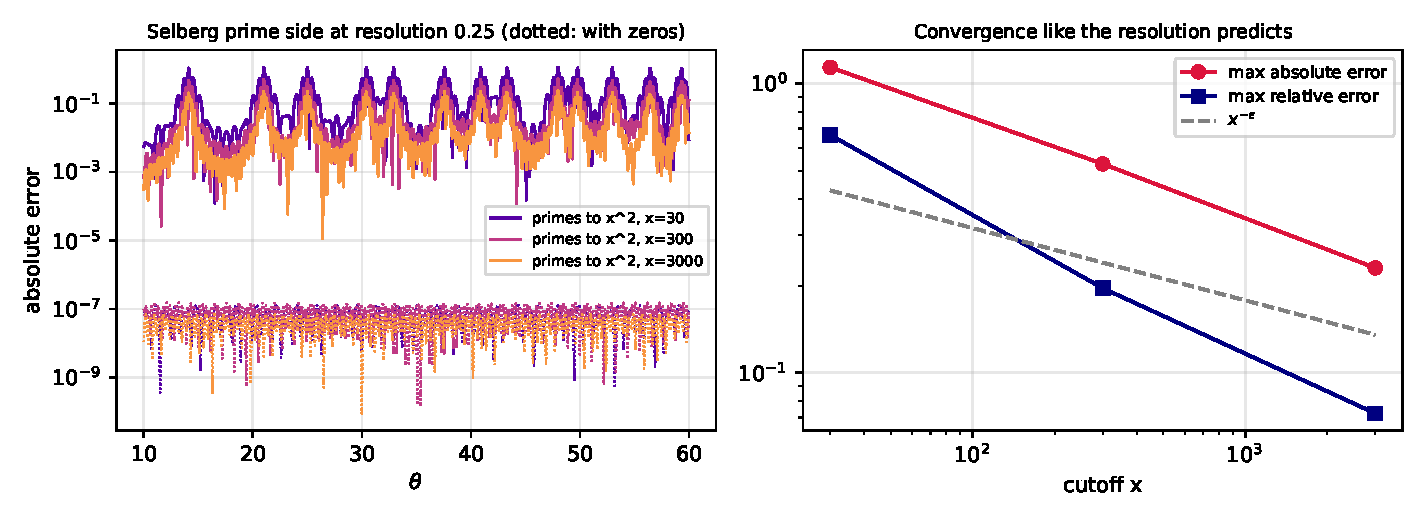
\includegraphics[width=\textwidth]{fig/selberg.pdf}
\caption{Left: absolute error of Selberg's smoothed prime side of $v_{3/4}$, at resolution $0.25$, for three cutoffs, and (dotted) with the sum over the first $1700$ zeros added. Right: the maximal absolute and relative errors against the cutoff, with $x^{-\varepsilon}$ for comparison.}
\label{fig:selberg}
\end{figure}

\subsection{Positivity: Brownian subordination and Weil's criterion}\label{sec:ch10:positivity}

The lemma cannot produce a Brownian first passage time to a random level from a positive input. Brownian motion with variance two per unit time first reaches a level $x>0$ at a time with Laplace transform $e^{-x\sqrt u}$, so its first passage time $T_Y$ to an independent level $Y\ge0$ has $\E e^{-uT_Y}=\E e^{-Y\sqrt u}$. The exponent $\log f(\alpha+s)/f(\alpha)=cs+\int(e^{-sx}+sx-1)L(dx)$ to which the lemma applies (Section~\ref{ch:clock}) would have to equal $-\log\E e^{-sY}$, which is concave in $s$ by H\"older's inequality, whereas $L\ge0$, $L\ne0$ makes it strictly convex, with second derivative $\int x^2e^{-sx}L(dx)>0$. With $c\ge0$ the lemma gives a GGC with Thorin density $(2\pi\sqrt z)^{-1}[c+\int2\sin^2(x\sqrt z/2)\,xL(dx)]$, but not a first passage time. Conversely, an infinitely divisible level with $\E e^{-sY}=\exp(-bs-\int(1-e^{-sx})\Pi(dx))$ enters the lemma with $c=b+\int x\,\Pi(dx)$ and the negative input $L=-\Pi$, and $T_Y$ receives the signed density $(2\pi\sqrt z)^{-1}[b+\int x\cos(x\sqrt z)\,\Pi(dx)]$. For a Poisson level ($\Pi=\delta_1$, $b=0$) this is $\cos(\sqrt z)/(2\pi\sqrt z)$, and $T_Y$ is not a GGC: it has an atom $e^{-1}$ at $0$. A positive input and a random level coexist only for pure drift, with transform $e^{-c\sqrt u}$ and Thorin density $c/(2\pi\sqrt z)$.

The reciprocal direction does work: for $Y\ge0$ infinitely divisible with finite mean $m$, $T_m\overset d=T_Y+R$, with $T_m$ the first passage time to the level $m$ and $R$ a GGC independent of $T_Y$, which for the clock is Proposition~\ref{tx:prop:W} and for a Barnes beta law is Proposition~\ref{tx3:prop:barnes}.

For $\xi$ there is no random level at any basepoint. By Stirling's formula and the polynomial growth of $\zeta$ in vertical strips, $|\xi(\alpha)/\xi(\alpha+it)|$ is at least $e^{\pi|t|/4}$ divided by a power of $|t|$, while $|\E e^{-itY}|\le1$; so $s\mapsto\xi(\alpha)/\xi(\alpha+s)$ is never a Laplace transform in $s$, although for $\alpha\ge1$ it is one in $u=s^2$ (Theorem~\ref{thm:poisson}). For $\alpha>1$ the input of $\xi$ is signed, and the positivity of $U_\alpha$ is created by the zeros through the Poisson kernels of Proposition~\ref{prop:struct}, not inherited from a positive input (Section~\ref{sec:ch6:consequences}); compare \cite[Remark 3.8]{P26}. At $\alpha=\tfrac12$ the obstruction is the drift zero case of Proposition~\ref{prop:nogo}, whose Brownian motion has variance one, and the curved boundaries of Section~\ref{ch:boundaries} take the place of the straight boundary with a random intercept. The obstruction concerns first passage alone (Section~\ref{ch:bphit}).

The same kernel puts Weil's criterion in variogram form. Section~\ref{ch:arith} defines the Thorin functional $U$ on the class $\mathcal T$ of functions $\varphi(z)=h(\sqrt z)$ with $h$ even, holomorphic on a strip $|\im r|\le\frac12+c$ for some $c>0$, and $O((1+|r|)^{-2-c})$ there. With $g(x)=\frac1{2\pi}\int h(r)e^{-irx}\,dr$,
\begin{equation}\label{eq:ch10:variogram}
\int_0^\infty\varphi(z)\,\frac{2\sin^2(x\sqrt z/2)}{2\pi\sqrt z}\,dz=g(0)-g(x),
\end{equation}
both sides being $\pi^{-1}\int_0^\infty h(r)(1-\cos xr)\,dr$. If $h\ge0$ on the real line, $g$ is positive definite and $g(0)-g(x)\ge0$ is a variogram. Weil's criterion \cite{Weil52} states that RH holds if and only if $\langle U,\varphi\rangle\ge0$ for every such $\varphi$, and by the explicit formula $U$ evaluates $\varphi$ at every zero. Formally, the lemma writes $\langle U,\varphi\rangle$ as the pairing of variograms with the canonical measure of \eqref{eq:split} taken at the centre, the measure $\nu$ of Section~\ref{ch:arith}, whose archimedean density and prime atoms are nonnegative and whose only negative input is the pole density $-e^{x/2}dx$. So RH says that on every variogram of a positive definite function the pole mass is dominated by the prime and archimedean mass. Both masses are infinite, and the absolutely convergent form of Section~\ref{ch:arith} makes the statement exact, the divergent constants cancelling through $\xi'(\tfrac12)=0$ (Section~\ref{sec:ch6:consequences}).

The linear programming formulation of \cite[Sections 18.2.8 and 18.2.9]{P26} works on this form, with the variograms as feasible directions. In a space of test functions of finite dimension the regularised domination is a feasibility problem with dual certificates, which Section~\ref{st:sec:wp5} proposes to solve at increasing dimension. Weil's criterion concerns $U$, which sees every zero, whereas the limit $\alpha\downarrow\tfrac12$ of the Thorin measures is $U_{\rm line}$, which pairs nonnegatively with every such $\varphi$ whatever the zeros do (Section~\ref{ch:arith}).
